\documentclass{article}


\usepackage{arxiv}

\usepackage[utf8]{inputenc} % allow utf-8 input
\usepackage[T1]{fontenc}    % use 8-bit T1 fonts
\usepackage{hyperref}       % hyperlinks
\usepackage{url}            % simple URL typesetting
\usepackage{booktabs}       % professional-quality tables
\usepackage{amsfonts}       % blackboard math symbols
\usepackage{nicefrac}       % compact symbols for 1/2, etc.
\usepackage{microtype}      % microtypography
\usepackage{lipsum}
\usepackage{graphicx}
\usepackage{multirow}

\title{Artist Identification	\\  a comparison between AlexNet, GoogLeNet and ResNeXt}


\author{
  Mattia Bottaro \\
  Dipartimento  di Matematica\\
  Università di Padova \\
  \texttt{mattia.bottaro@studenti.unipd.it} \\
  %% examples of more authors
   \And
  Mauro Carlin \\
Dipartimento  di Matematica\\
Università di Padova \\
\texttt{mauro.carlin@studenti.unipd.it} \\
  %% \AND
  %% Coauthor \\
  %% Affiliation \\
  %% Address \\
  %% \texttt{email} \\
  %% \And
  %% Coauthor \\
  %% Affiliation \\
  %% Address \\
  %% \texttt{email} \\
  %% \And
  %% Coauthor \\
  %% Affiliation \\
  %% Address \\
  %% \texttt{email} \\
}

\begin{document}
\maketitle

\begin{abstract}
	In this essay we present our work for the project of the Cognitive Services course.
	The problem we face is the artist identification task, that is given the image of a painting, being able to recognize its author.\\
	In order to resolve this task, we have exploit some differents Convolutional Neural Networks (CNNs) that comes with \textit{Pytorch} library. Such networks have been trained in according to two distinct approaches: \textit{1.} training them from scratch or  \textit{2.} exploit pre-trained models using transfer learning technique. We used the \textit{Google Cloud Plataform} to train and evaluate our models.\\
	What we have achieved is a set of results which are in line with  state-of-the-art (\cite{ArtistIdCNN406}) ..., confirming that CNNs are suitable to solve this type of task.
\end{abstract}


% keywords can be removed
\keywords{Convolutional Neural Networks \and Artist Identification \and CNNs \and ResNeXt \and GoogLeNet \and AlexNet \and Transfer Learning}


\section{Introduction}
Artist identification is a task regarding recognition of the painter who depicted a certain painting, given an image of it.\\
It's still nowadays a difficult problem to solve for the following reasons: \textit{1.} there are not many contributions yet and these rely on the latest models of deep learning (e.g. CNNs). \textit{2.} The available datasets are not as large as those used by models that solve more common tasks such as object detection or face recognition. \textit{3.} An artist's style can change a lot through his works, or it could be influenced by other painters. \\For example, it is well known that Paul Cézanne and Camille Pissarro, who have spent a period of their lives in close contact, have produced some works of similar style.\\
This type of task is still done by art experts and contributions to this type of problem can help and lead to \textit{1.} the development of automatic fake artifact detection and \textit{2.} automatic cataloguing of artworks.\\

We used three different CNNs: AlexNet (2012), GoogLeNet (2014) and ResNeXt (2016). For each of them, we have established two different ways of training: from scratch and with transfer learning  upon pre-trained version of such CNNs. Then we have observed and compared their performance. From our experiment we have obtained ... RISULTATI 82\% accuracy.\\

The rest of the essay is structured as follows: In section 2 we discuss (\textbf{METTI I REF}) similarities and differences between previous works and ours. In section 3 we explain which dataset we have used, how it was formed and which preprocessing and data augmentation techniques we have exploited. In section 4 we exhibit the CNNs' architectures and how we have trained them. In section 5 we show some details regarding the \textit{GCloud Compute Engine}'s configuration, the metrics used to assess the goodness of the models and the detailed results of this experiment. Finally, in section 6 we draw some conclusion and we outline some possibile future works which rely on our result.


\section{Related Works}


\section{Dataset}\label{dataset}
\subsection{Overview}\mbox{}\\
The first requirement to train a CNN for artist identification is a dataset, of paintings of different artist, as large as possible. For our project we obtain a dataset from \cite{ArtGANDataset}, which is a subset of the WikiArt Dataset. \\
The dataset contain about 19,000 images of 23 different artists, regarding very different styles, genres  and epochs. There are also three .csv files that labeled all the paintings for genre, style, and artist: for our work we have used only the last one.\\ \\
In order to obtain a balanced dataset, we decided to select randomly 450 paintings for each artist, so in the end our dataset consists of 10,350 total images. \\
The next step was to divied the entire dataset in training, validation and test set. \cite{ArtGANDataset} suggests a possibile partition, but we decided to create our own because there isn't a test set in their repository, and some paintings included in the training set are also in the validation set, 
fact that can create a distorted evaluation of our model during training. Therefore, we split the dataset in training, validation and test sets using a 80-10-10 division per artist, obtaining a training set of 360 paintings per artist, and a validation and test sets each of 45 paintings per artist.

\subsection{Preprocessing and Data augmentation}\mbox{}\\
CNNs require a precise size for the images passed in it, so we had to modify the paintings in the dataset, considering that they vary widely in shape and size.\\
So, first, we take a 224$\times$224 crop of each input images, next we zero-center and normalize them, with mean and standard deviation calculated for each of the three channels red, green and blue (they are RGB images).  \\
During training we also randomly horizontally flip the image with a probability of 50\%, and also take a random crop of it (not always the central pixels), for essentialy two reasons:
\begin{itemize}
	\item randomness create variety and can avoid overfit;
	\item we assumed that the style of an artist is present everywhere in the painting, so taking random crops do not influence the performance of our models.
\end{itemize}
Instead, for validation and test sets we always have taken a central crop, in order to obtain stable results not depending on crop position.

\section{Method}\label{method}
In our work we have considered three different CNNs: AlexNet, GoogLeNet and ResNeXt. Every network we use takes as input a
3$\times$224$\times$224 RGB image and outputs the scores for each of the 23 artists present in our dataset.
\\
For all of our networks, we use a softmax classifier with
cross-entropy loss:
\begin{equation}
L_{i}=-\log \left(\frac{e^{f_{y_{i}}}}{\sum_{j} e^{f_{j}}}\right)
\end{equation}
\textbf{SPIEGARE}

First, we have trained the networks from scratch, in order to allow the network to learn features solely for our specific task of artist identification. \\
Afterwards, starting from networks with weights pre-trained on ImageNet dataset, we trained them using transfer learning to understand if a feature representation from ImageNet is a valuable starting point for our problem.\\
In both approches, we replaced the last fully-connected layer of the CNNs with a new one to calculate a score for each artist in
our dataset. We used \cite{pytorchguide} as a guide for replacing the fully-connected layer, and for performing transfer learning on the pre-trained networks.

\subsection{AlexNet}
AlexNet was the winning entry in ILSVRC 2012. It solves the problem of image classification where the input is an image of one of 1000 different classes (e.g. cats, dogs etc.) and the output is a vector of 1000 numbers, achieving a top-5 error of 15,8\%.
Architecture (Figure \ref{fig:alexnet}) is made up of eight layers, five convolutional, some of them followed by max pooling layers, and three fully-connected, with ReLU as activation function.\\
AlexNet also uses dropout, introduced in 2012 in \cite{dropout}, to reduce overfitting. In dropout, a neuron is dropped from the network with a probability of 0.5. When a neuron is dropped, it does not contribute to either forward or backward propagation. 
As a result, the learnt weight parameters are more robust and do not get overfitted easily.\\
We decided to include AlexNet in our work because it represent the starting point of image classification with CNN, so it would be iteresting to compare its performance on our task with more recent, complex and deep networks.

\begin{figure}[h]
	\centering
	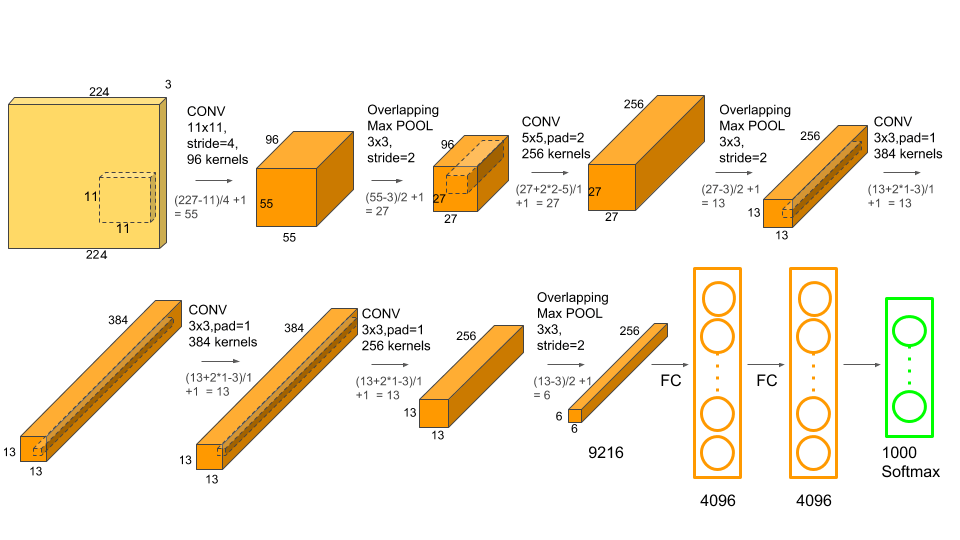
\includegraphics[width=0.7\linewidth]{image/AlexNet}
	\caption{AlexNet's architecture}
	\label{fig:alexnet}
\end{figure}

\subsection{GoogLeNet}
GoogLeNet won the ILSVRC 2014 achieving 6.67\% top-5 error on ImageNet. We considered this netowrk in our work PERCHè HA OTTENUTO IMPROVMENT NOTEVOLE DALL'ANNO PRECEDENTE, QUINDI INTRODUCENDO INNOVAZIONE CHE EFFETTI AMENTE FUNZONAO.
It is composed of 22 layers, with different innovations regarding the fully-connected layers, the vanishing gradient problem and a new inception module.\\
An interesting addition to the architecture is to change the second last fully-connected layer with an average pooling layer. This layer spatially averages the feature map, converting 7x7x1024 input to 1x1x1024, reducing the computation and the number of parameters, by a factor of 49. This average pooling layer is finally followed by a normal fully-connected layer with 1000 neurons (and 1024x1000 parameters), for the 1000 ImageNet classes.
During training, to address the vanishing gradient problem, special extra structures are added to the network (these are removed during testing). These are auxiliary classifiers attached to intermediate layers. All the losses from each classifier gets added up, taking contribution from the auxiliary classifier lower
than the main one, during training. The gradient from the main classifier which would have otherwise become very small, and thus slowing training, by time it reached the lower initial layers, receives gradient from the auxiliary classifiers and thus the net gradient becomes big enough to allow training to progress.
\begin{figure}[h]
	\centering
	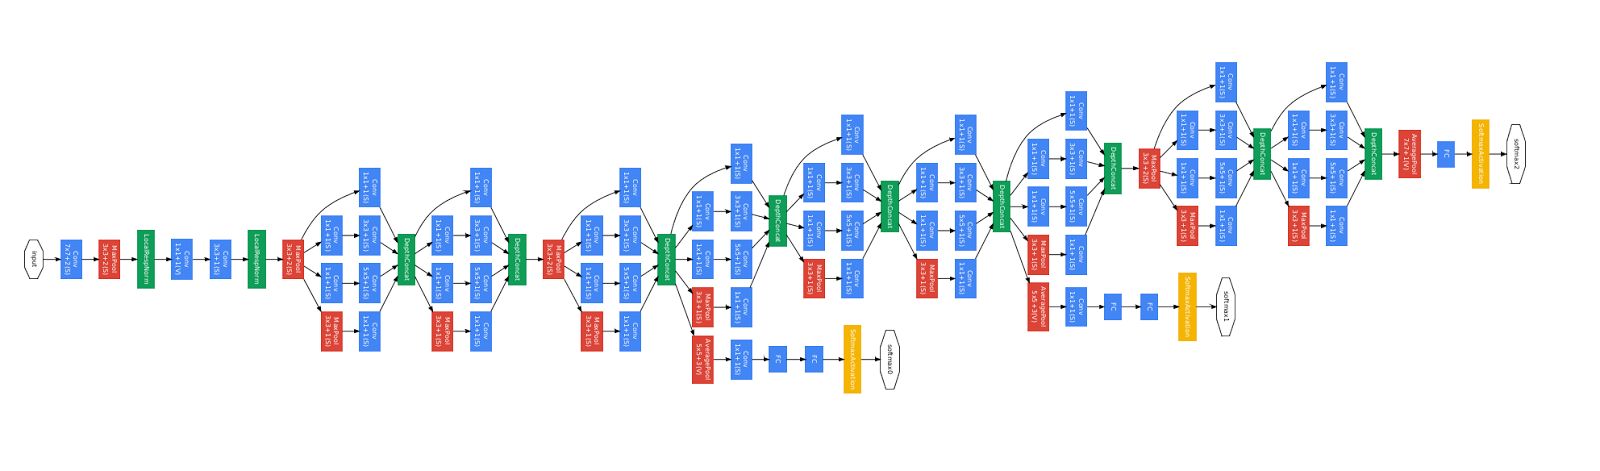
\includegraphics[width=0.7\linewidth]{image/GoogLeNet}
	\caption[]{GoogLeNet's architecture}
	\label{fig:googlenet}
\end{figure}

\subparagraph{Inception module}\mbox{}\\
Inception modules are used in GoogLeNet to allow for more efficient computation through a dimensionality reduction with stacked 1x1 convolutions. The modules were designed to solve the problem of computational expense, as well as overfitting, among other issues. The solution, in short, is to take multiple kernel filter sizes within the CNN, and rather than stacking them sequentially, ordering them to operate on the same level. 

As a neural net deals with a vast array of images, with wide variation in the featured image content, also known as the salient parts, they need to be designed appropriately. The most simplified version of an inception module works by performing a convolution on an input with not one, but three different sizes of filters (1x1, 3x3, 5x5). Also, max pooling is performed. Then, the resulting outputs are concatenated and sent to the next layer.
A method to reduce the number of computation is dimensionality reduction. This involves convolutions with 1x1 filters before convolutions with bigger filters.
\begin{figure}[h]
	\centering
	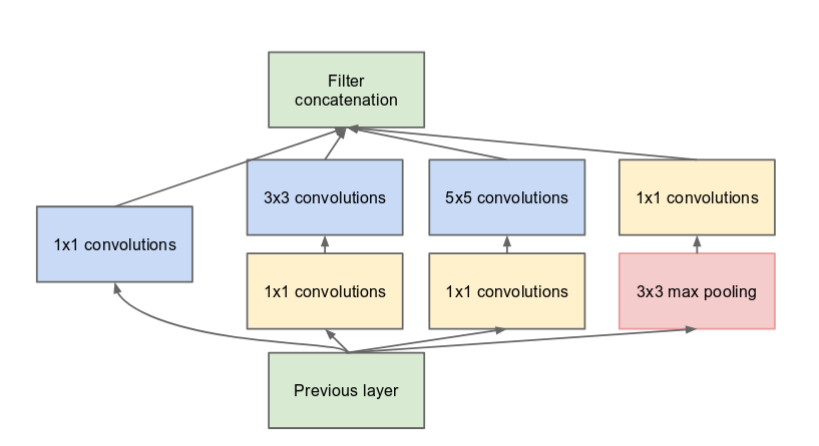
\includegraphics[width=0.7\linewidth]{image/inc_module}
	\caption{Inception module with dimension reduction}
	\label{fig:incmodule}
\end{figure}




\subparagraph{ResNeXt}
ResNeXt \cite{resnext} was the first runner up in ILSVRC 2016, achieving 3.03\% top-5 error rate, better than human precision on the same dataset (5,1\% error).The model name, ResNeXt, contains Next. It means the next dimension, on top of the ResNet, namely the winner in ILSVRC 2015. This next dimension is called the “cardinality” dimension.\\
The architecture adopts VGG/ResNets’ strategy of repeating layers, while
exploiting the split-transform-merge strategy (for example inception modules have the same approch, that is, input is split into a few lower-dimensional embeddings, transformed by a set of specialized filters, and merged by concatenation). 
A module in this network performs a set of transformations, each on a low-dimensional embedding, whose outputs are aggregated by summation. The transformations to be aggregated are all of the same topology (Figure \ref{fig:resnext_block} (right)).\\

\begin{figure}[h]
	\centering
	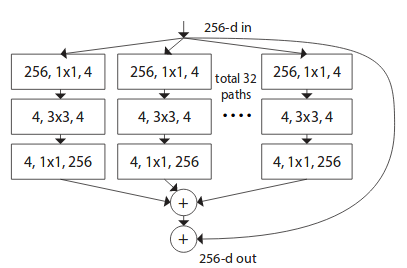
\includegraphics[width=0.7\linewidth]{image/resnext}
	\caption{Left: A block of ResNet. Right: A block of ResNeXt with cardinality=32. A layer is shown as (\# in channels, filter size, \# out channels)}
	\label{fig:resnext_block}
\end{figure}

Experiments in \cite{resnext} demonstrate that increasing cardinality (the size of the set of transformations) is a more effective way of gaining accuracy than going deeper or wider, especially when depth and width starts to give diminishing returns for existing models.\\
In our work we use ResNeXt-50 32$\times$4d (Figure \ref{fig:res}), that represents a network with four bottleneck, and each layer having cardinality of 32. 

\begin{figure}
	\centering
	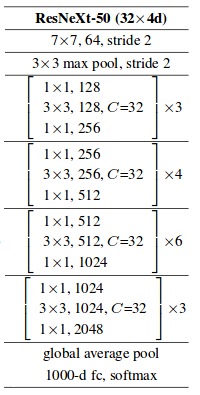
\includegraphics[height=0.4\linewidth]{image/res}
	\caption{ResNeXt-50 (32$\times$4)'s architecture}
	\label{fig:res}
\end{figure}


\section{Experiments}


\begin{table}[]
	\begin{tabular}{|c|c|c|c|c|}
		\hline
		\multicolumn{5}{|c|}{\textbf{Training from scratch}}                                                          \\ \hline
		\multirow{2}{*}{\textbf{Network}} & \multicolumn{2}{c|}{\textbf{Top-1}} & \multicolumn{2}{c|}{\textbf{Top-3}} \\ \cline{2-5} 
		& Train acc        & Test acc         & Train acc        & Test acc         \\ \hline
		AlexNet                           & 0.23103          & 0.27439          & 0.46159          & 0.51304          \\ \hline
		GoogLeNet                         & 0.42669          & 0.46956          & 0.68285          & 0.70628          \\ \hline
		ResNeXt-50                        & \textbf{0.50531} & \textbf{0.50048} & \textbf{0.74275} & \textbf{0.74782} \\ \hline
		ResNet-18 ref                     & 0,516            & 0,511            & 0,737            & 0,710            \\ \hline
	\end{tabular}
\end{table}

\paragraph{Setup}

\paragraph{Implementation Details}

\paragraph{Evaluation Metrics}

\paragraph{Results}




\section{Conclusion}

%%% Comment out this section when you \bibliography{references} is enabled.
\begin{thebibliography}{1}
	
	\bibitem{ArtistIdCNN406}
	Nitin Viswanathan.
	\newblock Artist Identification with Convolutional Neural Networks. \newblock 2017
	
	\bibitem{ArtGANDataset}
	Un qualche nome... \newblock
	\url{https://github.com/cs-chan/ArtGAN/tree/master/WikiArt Dataset}
	
	\bibitem{pytorchguide}
	Sasank Chilamkurthy.
	\url{https://pytorch.org/tutorials/beginner/transfer_learning_tutorial.html}
	
	\bibitem{dropout}
	G. E. Hinton, N. Srivastava, A. Krizhevsky, I. Sutskever and R. R. Salakhutdinov.
	Improving neural networks by preventing co-adaptation of feature detectors. 2012
	
	\bibitem{resnext}
	Saining Xie, Ross Girshick, Piotr Dollar, Zhuowen Tu, Kaiming He, UC San Diego, Facebook AI Research

	Aggregated Residual Transformations for Deep Neural Network. 2017
	
\end{thebibliography}


\end{document}

\end{document}